\documentclass[enabledeprecatedfontcommands,fontsize=11pt,paper=a4,twoside]{scrartcl}

\newcommand*{\red}{\textcolor{red}}
\newcommand*{\blue}{\textcolor{blue}}

\newcommand{\grad}{\ensuremath{^{\circ}} }
\renewcommand{\strut}{\vrule width 0pt height5mm depth2mm}

\usepackage[utf8]{inputenc}
\usepackage[T1]{fontenc}
\usepackage[final]{pdfpages}
% obere Seitenränder gestalten können
\usepackage{fancyhdr}
\usepackage{moreverb}
% Graphiken als jpg, png etc. einbinden können
\usepackage{graphicx}
\usepackage{stmaryrd}
% Floats Objekte mit [H] festsetzen
\usepackage{float}
% setzt URL's schön mit \url{http://bla.laber.com/~mypage}
\usepackage{url}
% Externe PDF's einbinden können
\usepackage{pdflscape}
% Verweise innerhalb des Dokuments schick mit " ... auf Seite ... "
% automatisch versehen. Dazu \vref{labelname} benutzen
\usepackage[ngerman]{varioref}
\usepackage[ngerman]{babel}
\usepackage{ngerman}
% Bibliographie
\usepackage{bibgerm}
\usepackage{svg}
% Tabellen
\usepackage{tabularx}
\usepackage{supertabular}
\usepackage[colorlinks=true, pdfstartview=FitV, linkcolor=blue,
            citecolor=blue, urlcolor=blue, hyperfigures=true,
            pdftex=true]{hyperref}
\usepackage{bookmark}



\newcounter{one}
\newcounter{two}[one]
\newcounter{three}[two]

\newcommand{\tone}{0\theone}
\newcommand{\ttwo}{0\thetwo}
\newcommand{\tthree}{0\thetree}
\newcommand{\one}{\stepcounter{one}0\theone}
\newcommand{\two}{\stepcounter{two}0\thetwo}
\newcommand{\three}{\stepcounter{three}0\thethree}
\newcommand\s{\rule{0pt}{4ex}}        
\newcommand{\cb}[1]{{\textcolor{blue}{#1}}}
\newcommand*{\hint}{\paragraph{\textcolor{blue}{Hinweise}}}
\newcommand*{\condition}{\paragraph{Voraussetzung}$\;$ \vspace{0.2cm}\\}
\newcommand*{\actions}{\paragraph{Vorgehen} $\;$\vspace{0.2cm}\\}
\newcommand*{\action}{\paragraph{Vorgehen}}
\newcommand*{\hdot}{\\ \hdashline[1pt/5pt]}
\newcommand*{\hdo}{.............}


\usepackage{geometry}
\usepackage{hyperref}
\usepackage{pdfpages} 
\usepackage{colortbl}
%\usepackage{graphicx}   
%\usepackage[utf8x]{inputenc}
\usepackage{fmtcount}
\usepackage[ngerman]{babel}
\usepackage{booktabs}
\usepackage{fancyhdr}
\usepackage[T1]{fontenc}
\usepackage{nameref}
\usepackage{graphicx}
\usepackage{subfigure}


\pagestyle{fancy}
\fancyhf{}

%

%

%

%

\definecolor{dartmouthgreen}{rgb}{0.05, 0.5, 0.06}
\definecolor{color}{rgb}{0.67, 0.88, 0.69}
\definecolor{todo}{rgb}{1.0, 0.41, 0.71}
\definecolor{sort}{rgb}{0.45, 0.76, 0.98}
\definecolor{prob}{rgb}{0.74, 0.83, 0.9}
\definecolor{anw}{rgb}{0.94, 0.86, 0.51}
\definecolor{ghostwhite}{rgb}{0.97, 0.97, 1.0}
\definecolor{glaucous}{rgb}{0.38, 0.51, 0.71}
\usepackage{amsmath}
\usepackage{tabularx}
\usepackage{setspace} 
\hypersetup{
	colorlinks = true,
	linkbordercolor = {white},
	linkcolor=dartmouthgreen,          % color of internal links (change box color with linkbordercolor)
	citecolor=red,        % color of links to bibliography
	filecolor=magenta,      % color of file links
	urlcolor=cyan 
}
\usepackage{geometry}
\geometry{
	a4paper,
	left=20mm,
	right=20mm,
	top=2cm,
	bottom=4cm,
	footskip=4cm
}


\addtolength{\headwidth}{20mm}
\addtolength{\headheight}{2\baselineskip}
\addtolength{\headheight}{0.61pt}


\renewcommand{\headrulewidth}{0pt}
\renewcommand{\headrule}{\vbox to 0pt{\rule{\headwidth}{0.2pt}}}
\setlength{\headsep}{30pt}


\hyphenation{Arbeits-paket}

% Damit Latex nicht zu lange Zeilen produziert:
%\sloppy
%Uneinheitlicher unterer Seitenrand:
%\raggedbottom

% Kein Erstzeileneinzug beim Absatzanfang
% Sieht aber nur gut aus, wenn man zwischen Absätzen viel Platz einbaut
%\setlength{\parindent}{0ex}

% Abstand zwischen zwei Absätzen
%\setlength{\parskip}{1ex}

% Seitenränder für Korrekturen verändern
%\addtolength{\evensidemargin}{-1cm}
%\addtolength{\oddsidemargin}{1cm}

%\bibliographystyle{gerapali}

% Lustige Header auf den Seiten
  \pagestyle{fancy}
  \setlength{\headheight}{70.55003pt}
  \fancyhead{}
  \fancyhead[LO,RE]{Software--Projekt 2\\ WiSe 2018/2019
  \\Architekturbeschreibung}
  \fancyhead[LE,RO]{Seite \thepage\\\slshape \leftmark\\\slshape \rightmark}

%
% Und jetzt geht das Dokument los....
%

\begin{document}

% Lustige Header nur auf dieser Seite
  \thispagestyle{fancy}
  \fancyhead[LO,RE]{ }
  \fancyhead[LE,RO]{Universität Bremen\\FB 3 -- Informatik\\
  Prof. Dr. Rainer Koschke \\TutorIn: Marcel Steinbeck}
  \fancyfoot[C]{}

% Start Titelseite
  \vspace{3cm}

  \begin{minipage}[H]{\textwidth}
  \begin{center}
  \bf
  \Large
  Software--Projekt 2 WiSe 2018/2019\\
  \smallskip
  \small
  VAK 03-BA-901.02\\
  \vspace{3cm}
  \end{center}
  \end{minipage}
  \begin{minipage}[H]{\textwidth}
  \begin{center}
  \vspace{1cm}
  \bf
  \Large Benutzerhandbuch\\
  \vspace{2cm}
  
\includegraphics[width=3.0in]{logo_graphit.png}

  
  \end{center}
 
  \end{minipage}
  \vfill
  \begin{minipage}[H]{\textwidth}
  \begin{center}
  \sf
  \begin{tabular}{lr}
  Anthony Mendil & antmen@tzi.de \\
  Bastian Rexhäuser & brexhaeu@tzi.de\\
  Clement Phung & clement1@tzi.de \\
  Jacky Philipp Mach & machja@tzi.de \\
  Jonah Jaeger & jjaeger@tzi.de \\
  Nina Unterberg & nin\_unt@tzi.de \\
  \end{tabular}
  \\ ~
  \vspace{2cm}
  \\
  \it Abgabe: 10. März 2019 --- Version 1.0\\ ~
  \end{center}
  \end{minipage}

% Ende Titelseite

% Start Leerseite

\newpage

  \thispagestyle{fancy}
  \fancyhead{}
  \fancyhead[LO,RE]{Software--Projekt \\  2018/2019
  \\Benutzerhandbuch}
  
  \fancyhead[LE,RO]{Seite \thepage\\\slshape \leftmark\\~}
  \fancyfoot{}
  \renewcommand{\headrulewidth}{0.4pt}
  \tableofcontents

\newpage

  \fancyhead[LE,RO]{Seite \thepage\\\slshape \leftmark\\\slshape \rightmark}

%%%%%%%%%%%%%%%%%%%%%%%%%%%%%%%%%%%%%%%%%%%%%%%%%%%%%%%%%%%%%%%%%%%%%%%%
%%%%%%%%%%%%%%%%%%%%%%%%%%%%%%%%%%%%%%%%%%%%%%%%%%%%%%%%%%%%%%%%%%%%%%
\section*{Vorwort}
Mit diesem Handbuch wird die Bedienung der Software GraphIT beschrieben. Diese Anwendung wurde im Rahmen des Moduls \glqq{Softwareprojekt 2} \grqq im Wintersemester 2018/19 entwickelt wurde und ist zur Erstellung, Editierung und Visualisierung von Wirkungsdiagrammen für den Syndromansatz entworfen. Eine Nutzung des Programmes für Zwecke, die von dem angedachten Einsatzbereich abweicht ist möglich. Allerdings wird in diesem Dokument nicht weiter auf eine solche Nutzung eingegangen. Bei dieser Nutzung, die nicht dem angedachten Einsatz entspricht, ist ferner zu berücksichtigen, dass eventuell gewisse Funktionen wünschenswert wären, die aufgrund der Anforderungen aus der Anwenungsdomäne, für die diese Software entwickelt wurde, jedoch bewusst nicht eingebaut wurden. Insbesondere sind hier die Regeln zu beachten, die für die Erstellung von Wirkungszusammenhängen gemäß des Syndromansatzes gelten. Bei der vorliegenden Software handelt es sich um eine Neu-Entwicklung. Somit existieren keinerlei Vorversionen, mit denen der Funktionsumfang oder die Bedienung der Software in diesem Dokument verglichen werden könnte. 

%%%%%%%%%%%%%%%%%%%%%%%%%%%%%%%%%%%%%%%%%%%%%%%%%%%%%%%%%%%%%%%%%%%%%%%%
%%%%%%%%%%%%%%%%%%%%%%%%%%%%%%%%%%%%%%%%%%%%%%%%%%%%%%%%%%%%%%%%%%%%%%
\section{Einführung}
\subsection{Adressierte Leser}
Dieses Handbuch richtet sich an alle Nutzer, die GraphIt für ihren bestimmungsgemäßen Einsatz verwenden möchten. Dieser umfasst die Erstellung, Bearbeitung und Auswertung von Wirkungszusammenhängen gemäß des Syndromansatzes. Die Software ist sowohl für Anfänger geeignet, die noch nie oder nur sehr selten mit einem vergleichbaren Programm gearbeitet haben, als auch für Fortgeschrittene und Experten, die über mehr Erfahrung in der Bedienung ähnlicher Software verfügen. Es existieren keine weiteren Benutzerhandbücher neben diesem Dokument. Dementsprechend finden sich in diesem Dokument auch für alle Nutzer der thematisierten Software Hinweise zur korrekten Verwendung der Software. Von dem Adressatenkreis des vorliegenden Dokuments wird die Kenntnis der Terminologie des Syndromansatzes erwartet.  
\subsection{Verwandte Dokumente}
Neben dem Benutzerhandbuch der Software Graphit, existiert ebenfalls ein Testprotokoll, welches die Entwickler erstellt haben, um die Korrektheit der Software zu garantieren. Außerdem eine Architekturbeschreibung die detaillierteren Einblick in die Architektur der Software gewährt. 
\subsection{Konventionen}
\begin{itemize}
	\item Wenn im Verlaufe des Dokumentes von einem Graphen die Rede ist, dann wird sich auf einen Syndromansatz bezogen.
\end{itemize}

\subsection{Informationen über die Verwendung des Dokuments}

\begin{itemize}
	\item Alle eingebundenen Screenshots in das Dokument wurden auf einem Computer mit einem Windows 10 Betriebssystem aufgenommen. Wenn ihre Darstellung der Software leicht von den gerade erwähnten Screenshots abweicht, bitten wir dies zu entschuldigen.
	\item Um die Software Graphit am Besten verstehen und anwenden zu können, empfehlen wir das Dokument an Anfang bis Ende durchzuarbeiten, da sich manche Einträge auf vorherige beziehen. 
\end{itemize}



%%%%%%%%%%%%%%%%%%%%%%%%%%%%%%%%%%%%%%%%%%%%%%%%%%%%%%%%%%%%%%%%%%%%%%
\newpage
\section{Installation und Starten des Programms} \label{sec:installation}

\subsection{Installationsvoraussetzungen}
\subsubsection{Java 8}
\red{TODO}

\subsection{Installationsanweisungen}
\begin{itemize}
	\item \red{TODO}
\end{itemize}
\subsection{Starten des Programms}
\red{TODO}

\newpage	
%%%%%%%%%%%%%%%%%%%%%%%%%%%%%%%%%%%%%%%%%%%%%%%%%%%%%%%%%%%%%%%%%%%%%		
\section{Benutzeroberfläche}
\subsection{Tasten-/ Mausbelegungen}

\begin{tabular} {|p{8cm}|p{8cm}|}
	\hline
	\rowcolor{glaucous}\multicolumn{2}{|l|} {\parbox{16cm}{\textbf{\textcolor{ghostwhite}{Maus-/ Tastenbelegungen}}} } \\ \hline\hline 	
	Drucken	& Ctrl + P \\ \hline
	Neue Datei	& Ctrl + N \\ \hline
	GXL importieren	& Ctrl + Shift + I \\ \hline
	Speichern unter	&	Ctrl + S \\ \hline
\end{tabular}


\subsection{Übersicht}
1\hdo..Sphäre hinzufügen -Button \\
2\hdo..Auswahl -Button \\
3\hdo..Sphäre entfernen \\
4\hdo..Sphäre vergrößern \\
5\hdo..Sphäre verkleinern \\
6\hdo..Sphäre Füllfarbe verändern  \\
7\hdo..Sphäre Schriftart verändern  \\
8\hdo..Sphäre Schriftgröße verändern \\
9\hdo..Sphäre layouten \\
10\hdo  Symptom hinzufügen \\
11\hdo  Symptom entfernen \\
12\hdo  Symptom vergrößern \\
13\hdo  Symptom verkleinern \\
14\hdo  Symptom Füllfarbe verändern \\
15\hdo  Symptom Randfarbe verändern \\
16\hdo  Symptom Form verändern \\
17\hdo  Symptome layouten \\
18\hdo  Symptome Schriftart verändern \\
19\hdo  Symptome Schriftgröße verändern \\
20\hdo  Ankerpunkte einblenden \\
21\hdo  Relation entfernen \\
22\hdo  Relation Ankerpunkte entfernen \\
23\hdo  Relation Farbe verändern \\
24\hdo  Relation Kantenart  verändern \\
25\hdo  Relation Typ verändern \\
26\hdo  nach Relationstyp filtern \\
27\hdo  nach Regex filtern \\
28\hdo  Übersichtsleiste \\
29\hdo  Zoom Fenster  \\
30\hdo  Vorlage\\
31\hdo  Maximale Anzahl von Graph- Elementen\\
34\hdo  Relationen erlauben \\
35\hdo Sperrende Elemente auswählen \\
36\hdo Zoom-leiste \\
37\hdo aktuelle Mausposition \\
38\hdo Bearbeiter Modus\\
39\hdo Ersteller Modus\\
40\hdo Analyse Modus\\
41\hdo Undo/ rückgängig machen\\
42\hdo redo/ wiederholen\\
43\hdo gehighlighte Elemente ein-/ausblenden\\
44\hdo Element highlighten\\
45\hdo Element aus dem Highlight entfernen\\
46\hdo Elemente ein-/ausblenden\\
47\hdo Element zum Fadeout hinzufügen\\
48\hdo Element aus Fadeout entfernen\\
49\hdo Neue Datei hinzufügen\\
50\hdo Datei öffnen\\
51\hdo GXL importieren\\
52\hdo Speichern unter\\
53\hdo Exportieren als PDF/ GXL/ Verlaufsprotokoll\\
54\hdo Drucken\\
55\hdo Sprache Benutzeroberfläche\\
56\hdo Sprache des Graphen\\
57\hdo Dokumentation\\
58\hdo über uns \\
59\hdo Graphmaße\\
60\hdo Vorgänger/ Nachfolger\\
61\hdo Anzahl\\
62\hdo Kürzester Weg/ alle Wege\\
63\hdo Analyse-Optionen: Pfeilketten, Konvergente/ Divergente Verzweigungen, Verzweigungen,\\ 		
\hspace*{1.7cm} Zyklen\\
64\hdo Verlaufsübersicht\\
65\hdo Liste der Logs synchronisieren\\
66\hdo Filtern nach dem Verlaufstyp\\

\begin{landscape}
	\begin{figure}
		\centering
		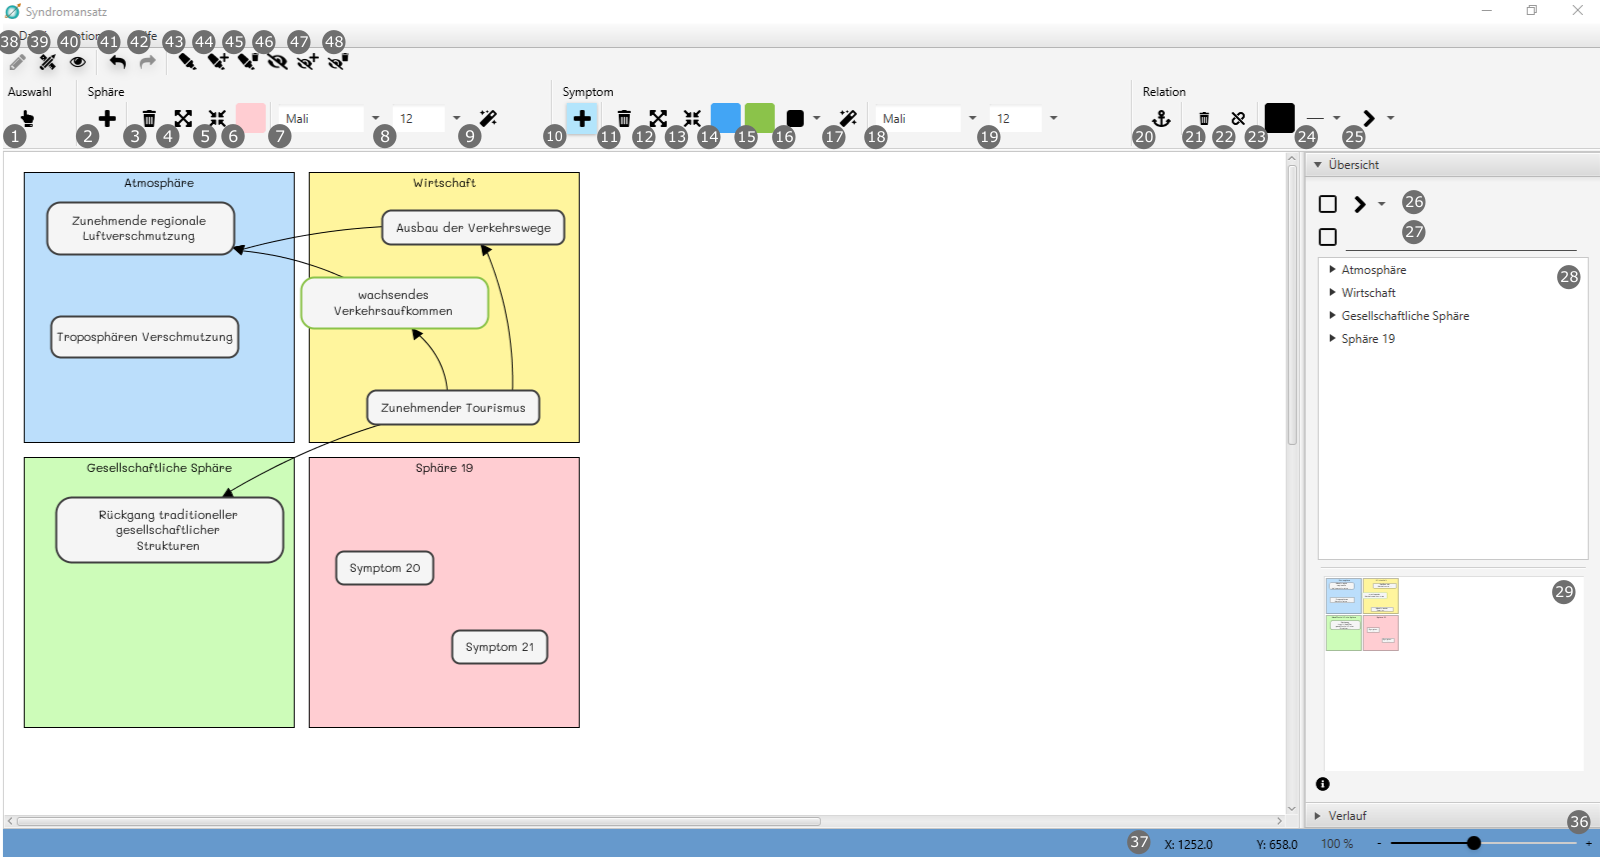
\includegraphics[width=22cm]{overview.png}
		\caption{Übersicht über den Ersteller Modus}
		\label{fig:label}
	\end{figure}
\end{landscape}
\begin{landscape}
	\begin{figure}
		\centering
		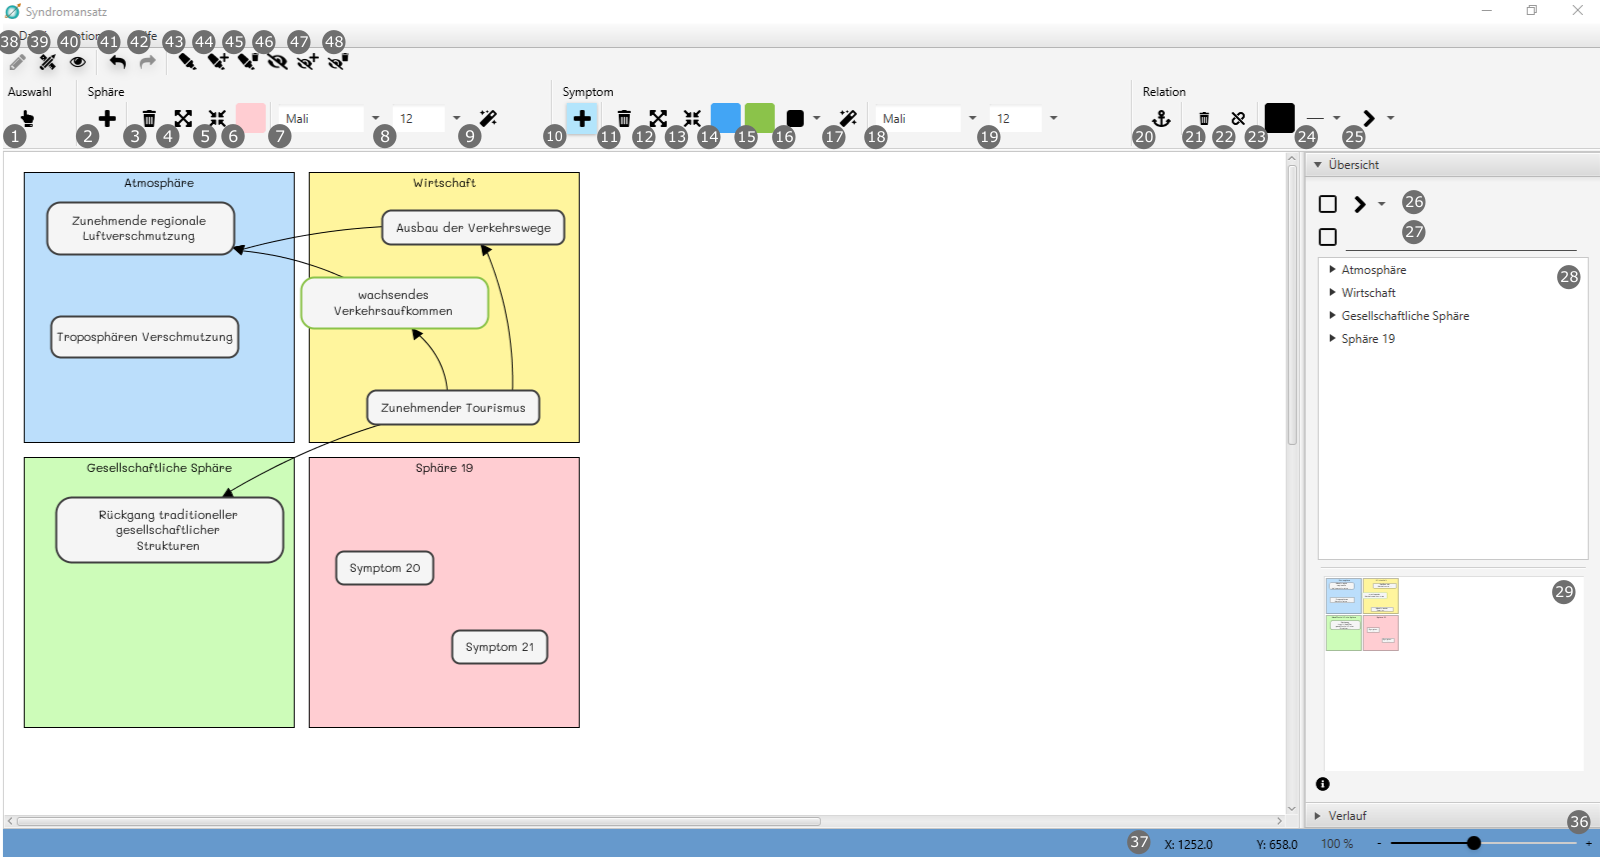
\includegraphics[width=22cm]{overview.png}
		\caption{Übersicht über den Analyse Modus}
		\label{fig:label}
	\end{figure}
\end{landscape}




\newpage	
%%%%%%%%%%%%%%%%%%%%%%%%%%%%%%%%%%%%%%%%%%%%%%%%%%%%%%%%%%%%%%%%%%%%%%	
\section{Übersicht} \label{sec:uebersicht}
\subsection{Ersteller Modus}
Im \texttt{Ersteller Modus} kann der Benutzer einen Syndromansatz erstellen und editieren. Im Unterschied zu dem \nameref{sec:editor} kann der Benutzer Vorlageregel für den aktuellen Syndromansatz hinterlegen. Diese werden erst auf dem Graphen im \nameref{sec:editor} angewandt. 


\subsubsection{Relevante Kapitel}
\begin{itemize}
	\item \nameref{pick}
	\item \nameref{edit}	
	\item \nameref{template}
	\item \nameref{overwiew}
	\item \nameref{zoom}
	\item \nameref{export}
	\item \nameref{import}
	\item \nameref{print}
	\item \nameref{dialog}
	\item \nameref{fehlermeldungen}
	\item \nameref{settings}	
\end{itemize}
\subsection{Bearbeiter Modus} \label{sec:editor}
Im \texttt{Bearbeiter Modus} kann der Benutzer einen Syndromansatz erstellen und bearbeiten. Die Bearbeitung des Graphen folgt den hinterlegten Vorlageregeln. Alle Aktionen auf dem Graph werden geloggt, d.h. ein Verlaufsprotokoll erstellt, welches ebenfalls einsehbar und exportierbar/ importierbar ist. 
\subsubsection{Relevante Kapitel}
\begin{itemize}
	\item \nameref{pick}
	\item \nameref{edit}	
	\item \nameref{logs}
	\item \nameref{overwiew}
	\item \nameref{zoom}
	\item \nameref{export}
	\item \nameref{import}
	\item \nameref{print}
	\item \nameref{dialog}
	\item \nameref{fehlermeldungen}
	\item \nameref{settings}	
\end{itemize}
\subsection{Analyse Modus}
Im \texttt{Analyse Modus} kann ein Syndromansatz analysiert und ausgewertet werden. In diesem Modus ist keine Bearbeitung des Graphen möglich. \\
Die Analyse umfasst z.B. die Lokalisierung von Pfeilketten oder die Berechnung des kürzesten Weges zwischen 2 Symptomen. \\
Die Auswertung der Nutzerinteraktionen ist ebenfalls möglich. Diese können gefiltert und angezeigt werden. 
\subsubsection{Relevante Kapitel}
\begin{itemize}
	\item \nameref{pick}	
	\item \nameref{logs}
	\item \nameref{overwiew}
	\item \nameref{zoom}
	\item \nameref{export}
	\item \nameref{import}
	\item \nameref{print}
	\item \nameref{dialog}
	\item \nameref{fehlermeldungen}
	\item \nameref{settings}	
	\item \nameref{analyse}
\end{itemize}

%%%%%%%%%%%%%%%%%%%%%%%%%%%%%%%%%%%%%%%%%%%%%%%%%%%%%%%%%%%%%%%%%%%%%%%

\newpage
\section{Instruktionen zur Nutzung des Programms} \label{sec:nutzung}
		\subsection{Auswahl von Graphelementen} \label{pick}
	\subsubsection{Eines Elements}
	\condition
	Es muss ein Syndromansatz mit mindestens einem Element (eine Sphäre/ ein Symptom/ eine Relation), welches ausgewählt werden soll, existieren. 
	\actions
	Alternative 1: 
	\begin{enumerate}
		\item In der Menüleiste den Button \textit{Auswahl} durch einen Links-Klick aktivieren. 
		\item Den Cursor auf das Element bewegen und die linke Maustaste klicken. 
	\end{enumerate}
	Alternative 2: 
	\begin{enumerate}
		\item In der Übersichtleiste das auszuwählende Element durch einen Links-Klick auswählen. 
	\end{enumerate}
	\hint
	\begin{itemize}
		\item Eine Relation kann manchmal etwas schwierig auszuwählen sein, da die Kanten vergleichsweise relativ dünn sind. 
	\end{itemize}
	
	\begin{figure}[ht!]
		\centering
		\subfigure[Alternative 1]{
			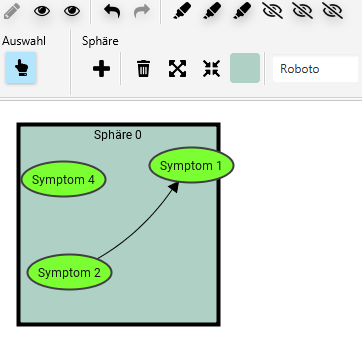
\includegraphics[width=0.4\columnwidth, keepaspectratio]{pick.png} 
		}
		\subfigure[Alternative 2]{
			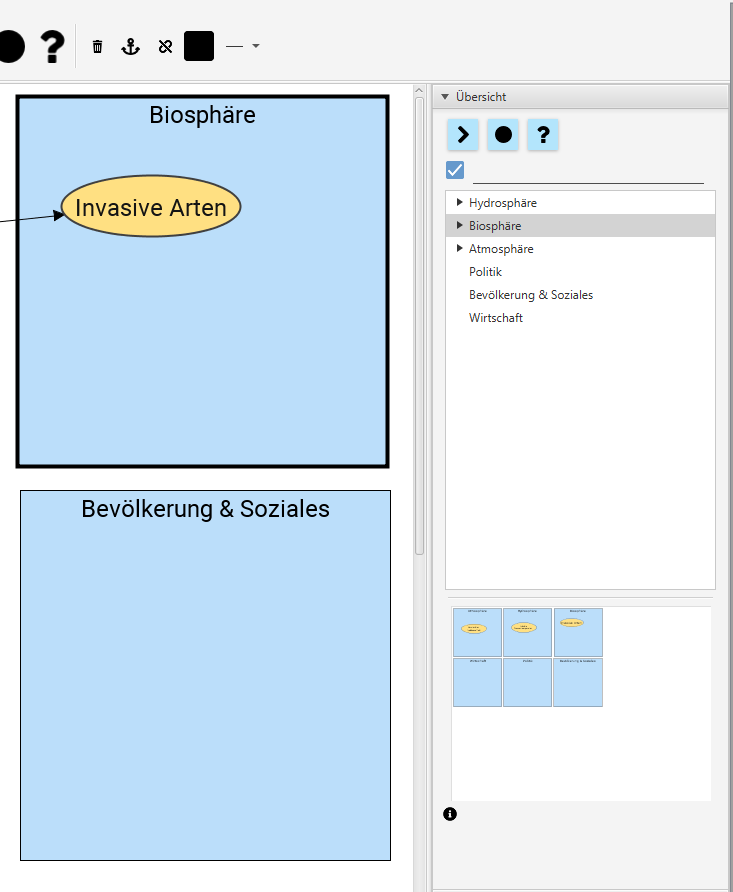
\includegraphics[width=0.4\columnwidth, keepaspectratio]{pick2.png} 
		}
		
	\end{figure}	
	%%%%%%%%%%%%%%%%%%%%%%%%%%%%%%%%%%%%%%%%%%%%%%%%%%%%%%%%%%%%%%%%%%%%%%% 	
	
	\newpage
	\subsubsection{Mehrerer Elemente}
	\condition
	Es muss ein Syndromansatz mit mindestens zwei Elemente (Sphären/ Symptome/ Relationen), welches ausgewählt werden soll, existieren. 
	\action
	\begin{enumerate}
		\item Auf der Tastatur den die Taste \texttt{Shift} gedrückt halten 
		\item Den Cursor auf das Element bewegen, welches zur Auswahl hinzugefügt werden soll und die linke Maustaste klicken. 
		\item Die \texttt{Shift} Taste solange gedrückt halten, wie Elemente der Auswahl hinzugefügt werden soll
		\item Die \texttt{Shift} Taste loslassen
	\end{enumerate}
	\hint
	\begin{itemize}
		\item Verschiedene Arten (Sphären/ Symptome/ Relationen) von Graphelementen können in einer Aktion der Auswahl hinzugefügt werden. \\ 
	\end{itemize}
%%%%%%%%%%%%%%%%%%%%%%%%%%%%%%%%%%%%%%%%%%%%%%%%%%%%%%%%%%%%
	\subsection{Editierung des Graphen}\label{edit}

		\hint
		\begin{itemize}
			\item In den folgenden Anleitungen wird immer davon ausgegangen, dass sich der Benutzer im \\
			Bearbeiter-/ Erstellermodus befindet und er somit die Berechtigung hat den Graphen zu editieren.
			\item Es wird vorausgesetzt, dass die Aktionen nicht durch die Vorlageregeln verhindert werden. D.h. das der Bearbeiter auf alle Elemente des Graphen freien Zugriff hat und alle Eigenschaften veränderbar sind.
		\end{itemize}
		\subsubsection{Undo/ Redo}
		Mit Undo/ Redo sind Aktionen auf dem Graphen wieder rückgängig zu machen oder rückgängig gemachte Aktionen erneut ausführbar. 
		\condition
		Es ist eine Aktions- Historie verfügbar. Beispiel: Es wurde ein Graph neu erstellt und eine Sphäre hinzugefügt. 	
		\action
		\begin{enumerate}
			\item Den Undo- Button durch einen Link-Klick auswählen. 
			\item Der Redo- Button sollte nun ebenfalls klickbar sein. Um die vorherige Aktion wieder auszuführen den Redo- Button klicken. 
		\end{enumerate}			
		
		\newpage	
		%%%%%%%%%%%%%%%%%%%%%%%%%%%%%%%%%%%%%%%%%%%%%%%%%%%%%%%%%%%%%%%%%%%%%%%%%%%%%%%%%%%%%%%%%%%%%%%%%%%%%%%%%%%%%	
		\subsubsection{Sphäre hinzufügen}	
		\condition 	
		Das Programm ist gestartet.
		\actions
		\begin{enumerate}
			\item In der Menüleiste den Button \textit{Sphäre hinzufügen} durch einen Links-Klick aktivieren.
			\item Den Cursor auf die gewünschte Position bewegen, an der sich keine andere Sphäre befindet, und auf die linke Maustaste klicken.
		\end{enumerate}
		\hint
		\begin{itemize}
			\item Es ist nicht möglich eine Sphäre auf einer anderen Sphäre hinzuzufügen. Wird dies versucht, wird keine neue Sphäre hinzugefügt und es erscheint eine Fehlermeldung.
	\end{itemize}
	
			\newpage	
		%%%%%%%%%%%%%%%%%%%%%%%%%%%%%%%%%%%%%%%%%%%%%%%%%%%%%%%%%%%%%%%%%%%%%%%%%%%%%%%%%%%%%%%%%%%%%%%%%%%%%%%%%%%%%	
		\subsubsection{Sphäre entfernen}
			\condition 	
		Ein Syndromansatz mit mindestens einer Sphäre ist im Programm geöffnet. 
		\actions  
		Alternative 1:
		\begin{enumerate}
			\item Die Sphäre, die gelöscht werden soll mit einem Links-Klick auswählen.
			\item Die \textit{Entfernen}-Teste der Tastatur drücken.
		\end{enumerate}
		Alternative 2:
			\begin{enumerate}
			\item Die Sphäre, die gelöscht werden soll mit einem Links-Klick auswählen.
			\item In der Menüleiste einen Links-Klick auf den Button \textit{Sphäre löschen} ausführen.
		\end{enumerate}
		Alernative 3:
		\begin{enumerate} 
			\item In diesem Kontextmenü der zu löschenden Sphäre die \textit{Entfernen}-Option mit einem Links-Klick auswählen.
		\end{enumerate}
		\hint
		\begin{itemize}
			\item Wird eine Sphäre gelöscht, so werden automatisch auch alle Symptome entfernt, die zu dieser Sphäre gehören. Damit werden dann auch alle Relationen gelöscht, die in einem dieser Symptome einmünden oder von einem dieser Symptome ausgehen.
		\end{itemize}
		
				\newpage	
		%%%%%%%%%%%%%%%%%%%%%%%%%%%%%%%%%%%%%%%%%%%%%%%%%%%%%%%%%%%%%%%%%%%%%%%%%%%%%%%%%%%%%%%%%%%%%%%%%%%%%%%%%%%%%	
		\subsubsection{Sphäre verschieben}
				\condition 	
		Ein Syndrom mit mindestens einer Sphäre ist im Programm geöffnet. 
		\actions  
		\begin{enumerate}
			\item Die Sphäre, die verschoben werden soll mit einem Rechts-Klick auswählen.
			\item Die (rechte) Taste gedrückt halten und den Cursor an eine Zielstelle bewegen, an der sich keine andere Sphäre befindet. Beim Bewegen des Cursors bewegt sich die Sphäre bereits mit. 
			\item Die rechte Maustaste loslassen.
		\end{enumerate}
		\hint
		\begin{itemize}
			\item Es ist nicht möglich, eine Sphäre zu verschieben, wenn sich an der Zielposition bereits eine andere Sphäre befindet. Wird dies versucht, wird die Sphäre nicht verschoben und es erscheint eine Fehlermeldung.
		\end{itemize}
		
				\newpage	
		%%%%%%%%%%%%%%%%%%%%%%%%%%%%%%%%%%%%%%%%%%%%%%%%%%%%%%%%%%%%%%%%%%%%%%%%%%%%%%%%%%%%%%%%%%%%%%%%%%%%%%%%%%%%%	
		\subsubsection{Größe der Sphäre verändern}
				\condition 	
		Ein Syndrom mit mindestens einer Sphäre ist im Programm geöffnet. 
		\actions  
		Alternative 1:
		\begin{enumerate}
			\item Die Sphäre, deren Größe verändert werden soll, mit einem Links-Klick auswählen.
			\item So oft die \glqq\textit{+}\grqq- / \glqq\textit{-}\grqq-Taste der Tastatur drücken bis die Sphäre die gewünschte Größe hat. \\(Nicht die \glqq\textit{+}\grqq- / \glqq\textit{-}\grqq-Taste des Nummernblocks)
		\end{enumerate}
		Alternative 2:
			\begin{enumerate}
			\item Die Sphäre, deren Größe geändert werden soll, mit einem Links-Klick auswählen.
			\item In der Menüleiste so oft  Links-Klick auf den Button \textit{Sphäre vergrößern}/\textit{Sphäre verkleinern} ausführen bis die Sphäre die gewünschte Größe hat.. 
		\end{enumerate}
		\hint
		\begin{itemize}
			\item Eine Sphäre kann nicht mehr verkleinert werden, wenn sie bereits ihre minimale Größe hat.
			\item Eine Sphäre kann nicht weiter vergrößert werden, wenn die Vergrößerung zu einer Überlappung von zwei Sphären führen würde.
			\end{itemize}
			
					\newpage	
		%%%%%%%%%%%%%%%%%%%%%%%%%%%%%%%%%%%%%%%%%%%%%%%%%%%%%%%%%%%%%%%%%%%%%%%%%%%%%%%%%%%%%%%%%%%%%%%%%%%%%%%%%%%%%	
		\subsubsection{Farbe der Sphäre ändern}
				\condition 	
		Ein Syndrom mit mindestens einer Sphäre ist im Programm geöffnet. 
		\actions  
		Alternative 1:
		\begin{enumerate}
			\item In der Menüleiste mit der linken Maustaste auf den Button \textit{Hintergrundfarbe der Sphäre verändern} klicken.
			\item Das Kontextmenü der Sphäre, deren Farbe geändert werden soll, öffnen und dort den Punkt \textit{Farbe} auswählen.
		\end{enumerate}
		Alternative 2:
		\begin{enumerate}
			\item Die Sphäre, deren Farbe geändert werden soll, mit einem Links-Klick auswählen.
			\item In der Menüleiste mit der linken Maustaste auf den Button \textit{Hintergrundfarbe der Sphäre verändern} klicken.
			\item In dem sich öffnenden Fenster die gewünschte Farbe mit einem Lnks-Klick auswählen.
		\end{enumerate}
		\hint
		\begin{itemize}
			\item Wenn die gewünschte Farbe nicht in dem sich öffnenden Fenster enthalten ist, lässt sich ein weiteres Farbwahl-Fenster durch einen Links-Klick auf \textit{Custom Color} öffnen. Dessen Bedienung ist im Kapiel -----XXX------ beschrieben.
	\end{itemize}	
	
			\newpage	
		%%%%%%%%%%%%%%%%%%%%%%%%%%%%%%%%%%%%%%%%%%%%%%%%%%%%%%%%%%%%%%%%%%%%%%%%%%%%%%%%%%%%%%%%%%%%%%%%%%%%%%%%%%%%%	
	\subsubsection{Titel der Sphäre ändern}
				\condition 	
		Ein Syndrom mit mindestens einer Sphäre ist im Programm geöffnet. 
		\actions  
		\begin{enumerate}
			\item Das Kontextmenü der Sphäre, deren Titel geändert werden soll, öffnen und dort die \textit{Titel}-Option mit einem Links-Klick auswählen. 
			\item In dem sich öffnenden Fenster für die gewünschten Sprache(n) den neuen Titel in die dafür vorgesehenen Felder eingeben.
			\item Die Änderung des Titels mit einem Links-Klick auf die \textit{Speichern}-Schaltfläche abschließen.
		\end{enumerate}
		\hint
		\begin{itemize}
			\item Der Titel einer Sphäre darf kein Semikolon enthalten.
		\end{itemize}
		\subsubsection{Contextmenü einer Sphäre öffnen/benutzen}
				\condition 	
		Ein Syndrom mit mindestens einer Sphäre ist im Programm geöffnet. 
		\actions  
		Alternative 1:
		\begin{enumerate}
			\item Auf einer Sphäre einen Rechts-Klick ausführen.
			\item Im sich öffnenden Kontextmenü die gewünschte Option mit einem Links-Klick auswählen.
		\end{enumerate}
		\hint
		\begin{itemize}
			\item Es ist egal, ob eine die Späre, deren Kontextmenü geöffnet werden soll, vor dem Rechts-Klick auf diese Sphäre mit einem Links-Klick ausgewählt worden ist oder nicht.
		\end{itemize}
		
				\newpage	
		%%%%%%%%%%%%%%%%%%%%%%%%%%%%%%%%%%%%%%%%%%%%%%%%%%%%%%%%%%%%%%%%%%%%%%%%%%%%%%%%%%%%%%%%%%%%%%%%%%%%%%%%%%%%%	
		\subsubsection{Schriftart/-größe der Beschriftung der Sphäre ändern}
				\condition 	
		Ein Syndrom mit mindestens einer Sphäre ist im Programm geöffnet. 
		\actions  
		Alternative 1:
		\begin{enumerate}
			\item Die Sphäre, für die die Schriftart/-größe geändert werden soll, mit einem Links-Klick auswählen.
			\item In der Menüleiste einen Links-Klick auf das Feld klicken, in dem de aktuelle Schriftart/-größe der Sphäre angezeigt wird.
			\item In dem Drop-Down-Menü die Schriftart/-größe auswählen, die die Beschriftung der Sphäre haben soll.
		\end{enumerate}
		Alternative 2:
			\begin{enumerate}
			\item In der Menüleiste einen Links-Klick auf das Feld klicken, in dem de aktuelle Schriftart/-größe der Sphäre angezeigt wird.
			\item In dem Drop-Down-Menü die Schriftart/-größe auswählen, die die Beschriftung der Sphäre haben soll.
			\item Das Kontextmenü der Sphäre öffnen, deren Schriftart/-größe geändert werden soll und dort die Option \textit{Schriftart}/\textit{Schriftgröße} auswählen.
		\end{enumerate}
		
				\newpage	
		%%%%%%%%%%%%%%%%%%%%%%%%%%%%%%%%%%%%%%%%%%%%%%%%%%%%%%%%%%%%%%%%%%%%%%%%%%%%%%%%%%%%%%%%%%%%%%%%%%%%%%%%%%%%%	
		\subsubsection{Sphären layouten}
				\condition 	
		Ein Syndrom mit mindestens einer Sphäre ist im Programm geöffnet. 
		\actions  
		\begin{enumerate}
			\item In der Menüleiste im Bereich Sphären auf den \textit{Automatische Anordnung}-Button mit Links-Klick klicken.
		\end{enumerate}
		\hint
		\begin{itemize}
			\item Es ist nicht möglich das Sphäre zu löschen, wenn die Position von mindestens einer Sphäre im Erstellermodus in den Vorlage-Regeln gelocked wurde.
			\end{itemize}
		
				\newpage	
		%%%%%%%%%%%%%%%%%%%%%%%%%%%%%%%%%%%%%%%%%%%%%%%%%%%%%%%%%%%%%%%%%%%%%%%%%%%%%%%%%%%%%%%%%%%%%%%%%%%%%%%%%%%%%	
		\subsubsection{Symptom hinzufügen}
		\condition 	
		Ein Syndrom mit mindestens einer Sphäre ist im Programm geöffnet. 
		\actions
		\begin{enumerate}
			\item In der Menüleiste den Button \textit{Symptom hinzufügen} durch einen Links-Klick aktivieren.
			\item Den Cursor auf die gewünschte Position innerhalb einer Sphäre bewegen, an der sich kein(e) andere(s) Symptom / Relation befindet, und auf die linke Maustaste klicken.
		\end{enumerate}
		\hint
		\begin{itemize}
			\item Es ist nicht möglich, ein Symptom auf einen anderem Symptom hinzuzufügen. Wird dies versucht, wird kein neues Symptom hinzugefügt und es erscheint eine Fehlermeldung.
			\item Es ist nicht möglich, ein Symptom außerhalb einer Sphäre hinzuzufügen. Wird dies versucht, wird kein neues Symptom hinzugefügt und es erscheint eine Fehlermeldung.
			\item Es ist nicht möglich ein Symptom auf einer Relation hinzuzufügen. Wird dies versucht, wird kein neues Symptom hinzugefügt und es erscheint eine Fehlermeldung.
		\end{itemize}

		\newpage	
		%%%%%%%%%%%%%%%%%%%%%%%%%%%%%%%%%%%%%%%%%%%%%%%%%%%%%%%%%%%%%%%%%%%%%%%%%%%%%%%%%%%%%%%%%%%%%%%%%%%%%%%%%%%%%	
		\subsubsection{Symptom entfernen}
				\condition 	
		Ein Syndrom mit mindestens einer Sphäre, die ein oder mehr Symptome enthält, ist im Programm geöffnet. 
		\actions
		\begin{enumerate}
			\item Das Symptom, das gelöscht werden soll mit einem Links-Klick auswählen. 
			\item Die \textit{Entfernen}-Taste der Tastatur drücken.
		\end{enumerate}
		Alternative 2:
		\begin{enumerate}
			\item Das Symptom, das gelöscht werden soll mit einem Links-Klick auswählen. 
			\item In der Menüleiste den \textit{Symptom löschen}-Button durch einen Links-Klick auslösen.
		\end{enumerate}
		\hint
		\begin{itemize}
			\item Es ist nicht möglich, ein Symptom zu löschen, wenn der Titel und/oder die Position und/oder der Style dieses Symptoms in den Vorlage-Regeln im Erstellermodus gelockt wurde. Wird dies versucht, wird das Symptom nicht gelöscht und es erscheint eine Fehlermeldung.
		\end{itemize}
		
				\newpage	
		%%%%%%%%%%%%%%%%%%%%%%%%%%%%%%%%%%%%%%%%%%%%%%%%%%%%%%%%%%%%%%%%%%%%%%%%%%%%%%%%%%%%%%%%%%%%%%%%%%%%%%%%%%%%%	
		\subsubsection{Symptom verschieben}
					\condition 	
		Ein Syndrom mit mindestens einer Sphäre, die ein oder mehr Symptome enthält, ist im Programm geöffnet. 
		\actions
		\begin{enumerate}
			\item Das Symptom, das verschoben werden soll mit einem Rechts-Klick auswählen. 
			\item Die rechte Maustaste gedrückt halten und den Cursor an die Stelle bewegen, an der es platziert werden soll.
		\end{enumerate}
		\hint
		\begin{itemize}
			\item Es ist nicht möglich, ein Symptom auf die Position eines anderen Symptoms zu verschieben. Wird dies versucht, wird das Symptom an seiner ursprünglichen Stelle platziert und es erscheint eine Fehlermeldung.
			\item Es ist nicht möglich, ein Symptom außerhalb einer Sphäre zu platzieren. Wird dies versucht, wird das Symptom an seiner ursprünglichen Stelle platziert und es erscheint eine Fehlermeldung.
			\item Es ist nicht möglich ein Symptom auf eine Relation zu verschieben. Wird dies versucht, wird das Symptom an seiner ursprünglichen Stelle platziert und es erscheint eine Fehlermeldung.
			\item Es ist nicht möglich, ein Symptom zu verschieben, wenn die Position des Symptoms in den Vorlage-Regeln gelockt wurde oder die aktuelle Anzahl an Symptomen in der Sphäre, in der das Symptom (neu) platziert werden soll, bereits der maximalen Anzahl an Symptomen entspricht, die im Erstellermodus in den Vorlage-Regeln für diese Sphäre eingestellt wurde. Wird dies versucht, wird das Symtom nicht verschoben und es erscheint eine Fehlermeldung.
		\end{itemize}
		
				\newpage	
		%%%%%%%%%%%%%%%%%%%%%%%%%%%%%%%%%%%%%%%%%%%%%%%%%%%%%%%%%%%%%%%%%%%%%%%%%%%%%%%%%%%%%%%%%%%%%%%%%%%%%%%%%%%%%	
		\subsubsection{Größe eines Symptoms verändern}
					\condition 	
		Ein Syndrom mit mindestens einer Sphäre, die ein oder mehr Symptome enthält, ist im Programm geöffnet. 
		\actions
		Alternative 1:
		\begin{enumerate}
			\item Das Symptom, dessen Größe verändert werden soll, mit einem Links-Klick auswählen. 
			\item Die \glqq\textit{+}\grqq- / \glqq\textit{-}\grqq-Taste der Tastatur so oft drücken bis das Symptom die gewünschte Größe erreicht hat. \\
			(Nicht die  \glqq\textit{+}\grqq- / \glqq\textit{-}\grqq-Taste des Nummernblocks)
		\end{enumerate}
				Alternative 2:
		\begin{enumerate}
			\item Das Symptom, dessen Größe verändert werden soll, mit einem Links-Klick auswählen. 
			\item  In der Menüleiste den \textit{Symptom vergrößern}- / \textit{Symptom verkleinern}-Button klicken so oft drücken bis das Symptom die gewünschte Größe erreicht hat.
		\end{enumerate}
		\hint
		\begin{itemize}
			\item Es ist nicht möglich, ein Symptom zu verkleinern, wenn es bereits seine minimale Größe hat.
			\item Es ist nicht möglich, ein Symptom zu vergrößern  / verkleinern, wenn die Größe des Symptoms in den Vorlage-Regeln im Erstellermodus gelockt wurde. Wird dies versucht, wird die Größe des Symptoms nicht geändert und es erscheint eine Fehlermeldung.
			\item Es ist nicht möglich ein Symptom zu vergrößern, wenn die Vergrößerung eine Überlappung mit anderen Symptomen zufolge hätte.
		\end{itemize}
		
				\newpage	
		%%%%%%%%%%%%%%%%%%%%%%%%%%%%%%%%%%%%%%%%%%%%%%%%%%%%%%%%%%%%%%%%%%%%%%%%%%%%%%%%%%%%%%%%%%%%%%%%%%%%%%%%%%%%%	
		\subsubsection{Füllfarbe eines Symptoms verändern}
		\condition 	
		Ein Syndrom mit mindestens einer Sphäre, die ein oder mehr Symptome enthält, ist im Programm geöffnet. 
		\actions
		Alternative 1:
		\begin{enumerate}
			\item In der Menüleiste mit der linken Maustaste auf den Button \textit{Hintergrundfarbe des Symptoms verändern} klicken.
			\item Mit einem Rechts-Klick auf das Symptom, dessen Farbe geändert werden soll, dessen Kontextmenü öffnen.
			\item im Kontextmenü den Punkt \textit{Füllfarbe} auswählen.
		\end{enumerate}
		Alternative 2:
		\begin{enumerate}
			\item In der Menüleiste mit der linken Maustaste auf den Button \textit{Hintergrundfarbe des Symptoms verändern} klicken.
			\item In dem sich öffnenden Fenster \textit{Costom Color} mit einem Lnks-Klick auswählen und in dem sich öffnenden Farbwahl-Fenster eine Farbe einstellen und diese mit der \textit{Enter}-Taste bestätigen.
			 \item Mit einem Rechts-Klick auf das Symptom, dessen Farbe geändert werden soll, dessen Kontextmenü öffnen.
			\item im Kontextmenü den Punkt \textit{Füllfarbe} auswählen.
		\end{enumerate}
		Alternative 3:
		\begin{enumerate}
			\item Das Symptom, dessen Farbe geändert werden soll, mit einem Links-Klick auswählen.
			\item In der Menüleiste mit der linken Maustaste auf den Button \textit{Hintergrundfarbe des Symptoms verändern} klicken.
			\item In dem sich öffnenden Fenster die gewünschte Farbe mit einem Lnks-Klick auswählen.
		\end{enumerate}
		Alternative 4:
			\begin{enumerate}
			\item Das Symptom, dessen Farbe geändert werden soll, mit einem Links-Klick auswählen.
			\item In der Menüleiste mit der linken Maustaste auf den Button \textit{Hintergrundfarbe des Symptoms verändern} klicken.
			\item In dem sich öffnenden Fenster \textit{Costom Color} mit einem Lnks-Klick auswählen und in dem sich öffnenden Farbwahl-Fenster eine Farbe einstellen und diese mit der \textit{Enter}-Taste bestätigen.
		\end{enumerate}
		\hint
		\begin{itemize}
			\item Die Bedienung des Farbwahl-Fensters, zu dem man über \textit{Custom Color} gelangt, ist im Kapiel -----XXX------ beschrieben.
			\item Es ist nicht möglich die Farbe eines Symptoms zu ändern, wenn der Style dieses Symptoms im Erstellermodus in den Vorlage-Regeln gelocked wurde. Wird dies versucht, wird die Sphäre nicht gelöscht und es erscheint eine Fehlermeldung.
	\end{itemize}	
	
			\newpage	
		%%%%%%%%%%%%%%%%%%%%%%%%%%%%%%%%%%%%%%%%%%%%%%%%%%%%%%%%%%%%%%%%%%%%%%%%%%%%%%%%%%%%%%%%%%%%%%%%%%%%%%%%%%%%%	
		\subsubsection{Randfarbe eines Symptoms verändern}
				\condition 	
		Ein Syndrom mit mindestens einer Sphäre, die ein oder mehr Symptome enthält, ist im Programm geöffnet. 
		\actions
		Alternative 1:
		\begin{enumerate}
			\item In der Menüleiste mit der linken Maustaste auf den Button \textit{Randfarbe des Symptoms verändern} klicken.
			\item Mit einem Rechts-Klick auf das Symptom, dessen Farbe geändert werden soll, dessen Kontextmenü öffnen.
			\item im Kontextmenü den Punkt \textit{Randfarbe} auswählen.
		\end{enumerate}
		Alternative 2:
		\begin{enumerate}
			\item In der Menüleiste mit der linken Maustaste auf den Button \textit{Randgrundfarbe des Symptoms verändern} klicken.
			\item In dem sich öffnenden Fenster \textit{Costom Color} mit einem Lnks-Klick auswählen und in dem sich öffnenden Farbwahl-Fenster eine Farbe einstellen und diese mit der \textit{Enter}-Taste bestätigen.
			 \item Mit einem Rechts-Klick auf das Symptom, dessen Farbe geändert werden soll, dessen Kontextmenü öffnen.
			\item im Kontextmenü den Punkt \textit{Randfarbe} auswählen.
		\end{enumerate}
		Alternative 3:
		\begin{enumerate}
			\item Das Symptom, dessen Farbe geändert werden soll, mit einem Links-Klick auswählen.
			\item In der Menüleiste mit der linken Maustaste auf den Button \textit{Randfarbe des Symptoms verändern} klicken.
			\item In dem sich öffnenden Fenster die gewünschte Farbe mit einem Lnks-Klick auswählen.
		\end{enumerate}
		Alternative 4:
			\begin{enumerate}
			\item Das Symptom, dessen Farbe geändert werden soll, mit einem Links-Klick auswählen.
			\item In der Menüleiste mit der linken Maustaste auf den Button \textit{Randfarbe des Symptoms verändern} klicken.
			\item In dem sich öffnenden Fenster \textit{Costom Color} mit einem Lnks-Klick auswählen und in dem sich öffnenden Farbwahl-Fenster eine Farbe einstellen und diese mit der \textit{Enter}-Taste bestätigen.
		\end{enumerate}
		\hint
		\begin{itemize}
			\item Die Bedienung des Farbwahl-Fensters, zu dem man über \textit{Custom Color} gelangt, ist im Kapiel -----XXX------ beschrieben.
			\item Es ist nicht möglich die Farbe eines Symptoms zu ändern, wenn der Style dieses Symptoms im Erstellermodus in den Vorlage-Regeln gelocked wurde. Wird dies versucht, wird die Sphäre nicht gelöscht und es erscheint eine Fehlermeldung.
	\end{itemize}	
	
					\newpage	
		%%%%%%%%%%%%%%%%%%%%%%%%%%%%%%%%%%%%%%%%%%%%%%%%%%%%%%%%%%%%%%%%%%%%%%%%%%%%%%%%%%%%%%%%%%%%%%%%%%%%%%%%%%%%%	
		\subsubsection{Titel eines Symptoms ändern}
		\condition 	
		Ein Syndrom mit mindestens einer Sphäre, die ein oder mehr Symptome enthält, ist im Programm geöffnet. 
		\actions  
		\begin{enumerate}
			\item Das Symptom, dessen Titel geändert werden soll mit einem Rechts-Klick anklicken, sodass sich dessen Kontext-Menü öffnet.
			\item Im Kontextmenü ganz oben \textit{Titel} mit einem Links-Klick auswählen. 
			\item In dem sich öffnenden Fenster für die gewünschten Sprache(n) den nuen Titel in die dafür vorgesehenen Felder eingeben.
			\item Die Änderung des Titels mit einem Links-Klick auf die \textit{Speichern}-Schaltfläche abschließen.
		\end{enumerate}
		\hint
		\begin{itemize}
			\item Der Titel eines Symptoms darf kein Semikolon enthalten.
		\end{itemize}
		
				\newpage	
		%%%%%%%%%%%%%%%%%%%%%%%%%%%%%%%%%%%%%%%%%%%%%%%%%%%%%%%%%%%%%%%%%%%%%%%%%%%%%%%%%%%%%%%%%%%%%%%%%%%%%%%%%%%%%	
		\subsubsection{Contextmenü eines Symptoms öffnen/benutzen}
				\condition 	
		Ein Syndrom mit mindestens einer Sphäre, die ein oder mehr Symptome enthält, ist im Programm geöffnet. 
		\actions  
		\begin{enumerate}
			\item Auf einem Symptom einen Rechts-Klick ausführen.
			\item im sich öffnenden Kontextmenü die gewünschte Option mit einem Links-Klick auswählen.
		\end{enumerate}
		\hint
		\begin{itemize}
			\item Es ist egal, ob eine das Symptom, dessen Kontextmenü geöffnet werden soll, vor dem Rechts-Klick auf dieses Symptom ausgewählt worden ist oder nicht.
		\end{itemize}
		
				\newpage	
		%%%%%%%%%%%%%%%%%%%%%%%%%%%%%%%%%%%%%%%%%%%%%%%%%%%%%%%%%%%%%%%%%%%%%%%%%%%%%%%%%%%%%%%%%%%%%%%%%%%%%%%%%%%%%	
		\subsubsection{Schriftart/-größe der Beschriftung des Symptoms ändern}
				\condition 	
		Ein Syndrom mit mindestens einer Sphäre, die ein oder mehr Symptome enthält, ist im Programm geöffnet. 
		\actions  
		Alternative 1:
		\begin{enumerate}
			\item Das Symptom, für das die Schriftart/-größe geändert werden soll, mit einem Links-Klick auswählen.
			\item In der Menüleiste einen Links-Klick auf das Feld klicken, in dem de aktuelle Schriftart/-größe des Symptoms angezeigt wird.
			\item In dem Drop-Down-Menü die Schrifart/-größe auswählen, die die Beschriftung des Symptoms haben soll.
		\end{enumerate}
		Alternative 2:
			\begin{enumerate}
			\item In der Menüleiste einen Links-Klick auf das Feld klicken, in dem de aktuelle Schriftart/-größe des Symptoms angezeigt wird.
			\item In dem Drop-Down-Menü die Schrifart/-größe auswählen, die die Beschriftung des Symptoms haben soll.
			\item Mit einem Rechts-Klick auf das Symptom klicken, dessen Schriftart/-größe geändert werden soll.
			\item In dem sich öffnenden Kontextmenü die Option \textit{Schriftart}/\textit{Schriftgröße} auswählen.
		\end{enumerate}
		\hint
		\begin{itemize}
			\item Es ist nicht möglich die Schriftart/-größe eines Symptoms zu ändern, wenn der Style dieses Symptoms im Erstellermodus in den Vorlage-Regeln gelocked wurde. Wird dies versucht, wird die Schriftart/-größe nicht geändert und es erscheint eine Fehlermeldung.
			\end{itemize}
			
							\newpage	
		%%%%%%%%%%%%%%%%%%%%%%%%%%%%%%%%%%%%%%%%%%%%%%%%%%%%%%%%%%%%%%%%%%%%%%%%%%%%%%%%%%%%%%%%%%%%%%%%%%%%%%%%%%%%%	
			\subsubsection{Form eines Symptoms verändern}
							\condition 	
		Ein Syndrom mit mindestens einer Sphäre, die ein oder mehr Symptome enthält, ist im Programm geöffnet. 
		\actions
		\begin{enumerate}
			\item Das Symptom, dessen Form geändert werden soll mit einem Rechts-Klick auswählen. 
			\item In der Menüleiste den Button \textit{Form des Symptoms verändern} anklicken.
			\item In dem sich öffnenden Drop-Down-Menü die Form auswählen, die das Symptom haben soll.
		\end{enumerate}
		\hint
		\begin{itemize}
			\item Es ist nicht möglich, die Form eines Symptoms zu ändern, wenn der Style dieses Symptoms in den Vorlage-Regeln gelockt wurde. Wird dies versucht, wird die Form des Symtoms nicht geändert und es erscheint eine Fehlermeldung.
		\end{itemize}
		\subsubsection{Symptome layouten}
				\condition 	
		Ein Syndrom mit mindestens zwei Symptome, die in derselben oder in zwei verschiedenen Sphären enthalten sind und durch eine Relation verbunden sind, ist im Programm geöffnet. 
		\actions  
		\begin{enumerate}
			\item In der Menüleiste im Bereich Symptom auf den \textit{Automatische Anordnung}.Button mit Links-Klick klicken.
		\end{enumerate}

			
			\newpage	
		%%%%%%%%%%%%%%%%%%%%%%%%%%%%%%%%%%%%%%%%%%%%%%%%%%%%%%%%%%%%%%%%%%%%%%%%%%%%%%%%%%%%%%%%%%%%%%%%%%%%%%%%%%%%%	
		\subsubsection{Relation hinzufügen}
		\condition
		Um eine Relation hinzufügen zu können, müssen mindestens 2 Symptome im Syndromansatz existieren. 
		\action
		\begin{enumerate}
			\item Auf ein Symptom klicken und die Maustaste gedrückt halten.
			\item Die Maus zu einem zweiten Symptom bewegen. 
			\item Die Maustaste auf einem anderem Symptom loslassen. 
		\end{enumerate}
		\hint
		\begin{itemize}
			\item Die Darstellung (Farbe, Kantenart, Typ) der Relation wird aus den ausgewählten Werten auf der Benutzeroberfläche ermittelt. 
			\item Es können nur Relationen zwischen zwei Symptomen hinzugefügt werden. 
			\item Ein Symptom kann keine Relation auf sich selber haben.
			\item Die Ankerpunkte der Relationen (von dem ausgehenden/ eingehenden Symptom) werden automatisch gesetzt und können manuell durch den Benutzer im Nachhinein verändert werden. 
			\item Die Pfeile von Relationen des gleichen Typs werden dabei in einem bestimmten Bereich zusammengefasst dargestellt. 
			\item Pfeilspitzen verschiedenen Types sollen sich nicht überlappen.
		\end{itemize}
		
		\begin{figure}[ht!]
			\centering
			\subfigure[Alternative 1]{
				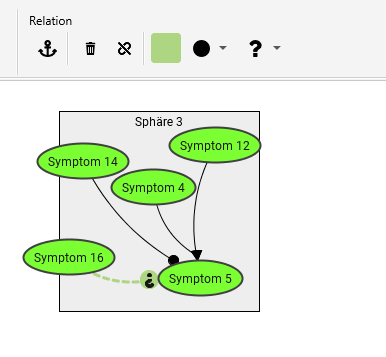
\includegraphics[width=0.4\columnwidth, keepaspectratio]{edge.png} 
			}			
		\end{figure}
		
		\newpage
		%%%%%%%%%%%%%%%%%%%%%%%%%%%%%%%%%%%%%%%%%%%%%%%%%%%%%%%%%%%%%%%%%%%%%%%%%%%%%%%%%%%%%%%%%%%%%%%%%%%%%%%%%%%%%
		\subsubsection{Relation entfernen}
		\condition
		Es muss mindestens eine Relation in dem Syndromansatz existieren. 
		\actions
		Alternative 1:
		\begin{enumerate}
			\item Die Relation, die gelöscht werden soll mit einem Links-Klick auswählen.
			\item Die \textit{Entfernen}-Taste der Tastatur drücken.
		\end{enumerate}
		Alternative 2:
		\begin{enumerate}
			\item Die Relation, welche gelöscht werden soll mit einem Links-Klick auswählen.
			\item In der Menüleiste einen Links-Klick auf den Button \textit{Relation entfernen} ausführen.
		\end{enumerate}
		Alternative 3:
		\begin{enumerate}
			\item Mit einem Rechts-Klick auf die Relation, welche gelöscht werden soll, das Kontextmenü öffnen. 
			\item In diesem Kontextmenü die \textit{Entfernen}-Option mit einem Links-Klick auswählen.
		\end{enumerate}
		
		
		%%%%%%%%%%%%%%%%%%%%%%%%%%%%%%%%%%%%%%%%%%%%%%%%%%%%%%%%%%%%%%%%%%%%%%%%%%%%%%%%%%%%%%%%%%%%%%%%%%%%%%%%%%%%%
		\subsubsection{Ankerpunkte ein-/ ausblenden}
		Ankerpunkte bezeichnen die Postion, wo die Relation in einem Symptom mündet/ von ihm ausgeht. Bei der Erstellung einer Relation werdend diese automatisch gesetzt und sind veränderbar. Das bedeutet, dass wenn ein Symptom bewegt wird, sich die Postion der Mündung/Ausgang der Relation in/aus das Symptom entsprechend anpasst und bewegt. Um das zu verhindert, können die Ankerpunkte manuell besetzt werden. Diese sind dann fest, d.h. auch beim Bewegen eines Symptoms bleibt die Position der Mündung/ Ausgang bestehen.
		\condition
		Es muss mindestens eine Relation im Syndromansatz existieren und mindestens ein Ankerpunkt gesetzt sein. 
		\action
		\begin{enumerate}
			\item In der Menüleiste den Button Ankerpunkte ein-/ausblenden durch einen Links- Klick aktivieren.
			\item Zum Ausblenden den Button durch einen Links- Klick deaktivieren. 
		\end{enumerate}
		\hint
		\begin{itemize}
			\item Die Ankerpunkte werden beim Einblenden rot eingefärbt. 
		\end{itemize}
		\begin{figure}[ht!]
			\centering
			\subfigure[Alternative 1]{
				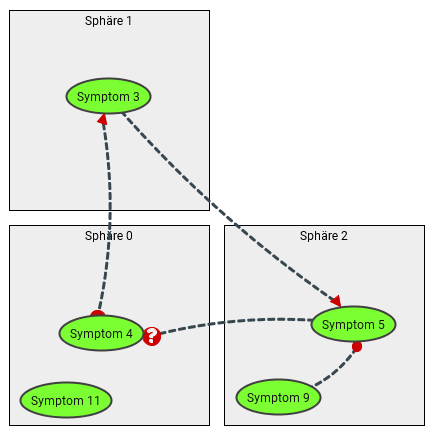
\includegraphics[width=0.4\columnwidth, keepaspectratio]{anchor.png} 
			}			
		\end{figure}
		
		\newpage
		%%%%%%%%%%%%%%%%%%%%%%%%%%%%%%%%%%%%%%%%%%%%%%%%%%%%%%%%%%%%%%%%%%%%%%%%%%%%%%%%%%%%%%%%%%%%%%%%%%%%%%%%%%%%%	
		\subsubsection{Ankerpunkte hinzufügen}
		\condition
		Es muss mindestens eine Relation im Syndromansatz existieren.
		\action
		\begin{enumerate}
			\item Die Kante durch einen Rechts- Klick auswählen und gedrückt halten.
			\item Befindet sich die Position der Maus beim Klick näher am Symptom, in welches die Relation mündet, wird der Ankerpunkt der Mündung der Relation gesetzt. Befindet sich die Postion der Maus beim Klick näher am Symptom, von dem die Kante ausgeht, wird der Ankerpunkt für den Ausgang der Kante gesetzt. 
			\item Die Kante in die gewünschte Richtung bewegen. Die Mündung/ der Ausgang der Kante wandert entsprechend mit. 
			\item Wenn die gewünschte Position erreicht ist, die gedrückte Maustaste loslassen. 
		\end{enumerate}
		\begin{figure}[ht!]
			\centering
			\subfigure[Alternative 1]{
				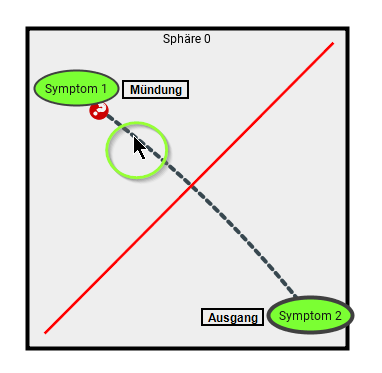
\includegraphics[width=0.3\columnwidth, keepaspectratio]{add_anchor.png} 
			}			
		\end{figure}
		\hint
		\begin{itemize}
			\item Beim Beispiel in der Abbildung wird aufgrund der Mausposition der Ankerpunkt bei der Mündung der Relation gesetzt.
		\end{itemize}
		
		%%%%%%%%%%%%%%%%%%%%%%%%%%%%%%%%%%%%%%%%%%%%%%%%%%%%%%%%%%%%%%%%%%%%%%%%%%%%%%%%%%%%%%%%%%%%%%%%%%%%%%%%%%%%%
		\subsubsection{Ankerpunkte entfernen}
		\condition
		Es muss mindestens eine Relation im Syndromansatz existieren.
		\action
		\begin{enumerate}
			\item Die gewünschte Relation durch einen Link- Klick auswählen. 
			\item In der Menüleiste einen Links-Klick auf den Button \textit{Ankerpunkt entfernen} ausführen.
		\end{enumerate}
		\hint
		\begin{itemize}
			\item Beim Entfernen der Ankerpunkte werden immer (wenn gesetzt) Ankerpunkte entfernt.\\
		\end{itemize}
		
		%%%%%%%%%%%%%%%%%%%%%%%%%%%%%%%%%%%%%%%%%%%%%%%%%%%%%%%%%%%%%%%%%%%%%%%%%%%%%%%%%%%%%%%%%%%%%%%%%%%%%%%%%%%%%
		\subsubsection{Farbe einer Relation verändern}
		\condition
		Es muss mindestens eine Relation im Syndromansatz existieren.
		\actions
		Alternative 1:
		\begin{enumerate}
			\item In der Menüleiste mit der linken Maustaste auf den Button \textit{Farbe der Relation verändern} klicken.
			\item Mit einem Rechts-Klick auf die Relation, deren Farbe geändert werden soll, ihr Kontextmenü öffnen.
			\item im Kontextmenü den Punkt \textit{Farbe} auswählen.
		\end{enumerate}
		Alternative 2:
		\begin{enumerate}
			\item Die Relation, deren Farbe geändert werden soll, mit einem Links-Klick auswählen.
			\item In der Menüleiste mit der linken Maustaste einen Links-Klick auf den Button \textit{Farbe der Relation verändern} ausführen.
			\item In dem sich öffnenden Fenster die gewünschte Farbe mit einem auswählen.
		\end{enumerate}	
		
		\newpage
		%%%%%%%%%%%%%%%%%%%%%%%%%%%%%%%%%%%%%%%%%%%%%%%%%%%%%%%%%%%%%%%%%%%%%%%%%%%%%%%%%%%%%%%%%%%%%%%%%%%%%%%%%%%%%
		\subsubsection{Type einer Relation verändern}
		\condition
		Es muss mindestens eine Relation im Syndromansatz existieren.
		\actions
		Alternative 1:
		\begin{enumerate}
			\item In der Menüleiste mit der linken Maustaste auf den Button \textit{Typ der Relation verändern} klicken.
			\item Mit einem Rechts-Klick auf die Relation, deren Typ geändert werden soll, ihr Kontextmenü öffnen.
			\item Im Kontextmenü den Punkt \textit{Typ} auswählen.
		\end{enumerate}
		Alternative 2:
		\begin{enumerate}
			\item Die Relation, deren Typ geändert werden soll, mit einem Links-Klick auswählen.
			\item In der Menüleiste mit der linken Maustaste einen Links-Klick auf den Button \textit{Typ der Relation verändern} ausführen.
			\item Aus dem Drop-Down einen Typ per Links- Klick auswählen. 
		\end{enumerate}	
		\hint
		\begin{itemize}
			\item Die normale Pfeilspitze stellt die verstärkende Beziehung von Relationen im Syndromansatz dar
			\item Die kreisförmige Pfeilspitze stellt die abschwächend Beziehung von Relationen im Syndromansatz dar
			\item Die Pfeilspitze mit dem Fragezeichen stellt die neutrale Beziehung von Relationen im Syndromansatz dar
		\end{itemize}
		
				\newpage
		%%%%%%%%%%%%%%%%%%%%%%%%%%%%%%%%%%%%%%%%%%%%%%%%%%%%%%%%%%%%%%%%%%%%%%%%%%%%%%%%%%%%%%%%%%%%%%%%%%%%%%%%%%%%%
		\subsubsection{Graphelemente hervorheben}
		\condition 	
		Ein Syndrom mit mindestens einer Sphäre, die ein oder mehr Symptome und eine oder mehr Relationen enthält, ist im Programm geöffnet. 
		\actions
		Alternative 1:
		\begin{enumerate}
			\item Das Symptom / die Relation, das / die hervorgehoben werden soll, mit einem Links-Klick auswählen. 
			\item In der Menüleiste den Button \textit{Elemente hervorheben} klicken.
		\end{enumerate}
				Alternative 2:
		\begin{enumerate}
			\item Im Kontextmenü des Graphelements, das hervorgehoben werden soll, die Option \textit{Hervorhebung} mit einem Links-Klck auswählen.
		\end{enumerate}
		\hint
		\begin{itemize}
					\item Es können lediglich Symptome und Relationen und somit keine Sphären hervorgehoben werden
					\item Wird die Aktion auf einem Graphelement ausgeführt, das aktuell bereits hervorgehoben ist, passiert nichts.
					\item Um die Hervorhebung zu aktivieren / sichtbar zu machen den Button \textit{Hervorgehobene Elemente aktivieren} in der Menüleiste anklicken. Durch einen erneuten Klick auf diesen Button wird die Hervorhebung wieder deaktiviert. Dabei kann dieser \textit{Hervorgehobene Elemente aktivieren}-Button zu einem beliebigen Zeitpunkt im oben beschriebenen Ablauf geklickt werden.
					\item Es können mehrere Symptome und Relationen ausgewählt werden, die anschließend durch Klicken des \textit{Elemente hervorheben}-Button hervorgehoben werden, indem die \textit{Shift}-Taste gedrückt gehalten wird und die gewünschten Elemente jeweils mit einem Links-Klick ausgewählt werden.
		\end{itemize}
		
			\newpage
		%%%%%%%%%%%%%%%%%%%%%%%%%%%%%%%%%%%%%%%%%%%%%%%%%%%%%%%%%%%%%%%%%%%%%%%%%%%%%%%%%%%%%%%%%%%%%%%%%%%%%%%%%%%%%
		\subsubsection{Graphelemente zur Hervorhebung hinzufügen}
				\condition 	
		Ein Syndrom mit mindestens einer Sphäre, die ein oder mehr Symptome und eine oder mehr Relationen enthält, ist im Programm geöffnet. Es ist mindestens eines dieser Elemente hervorgehoben und eines noch nicht hervorgehoben.
		\actions
		Das Graphelement, das neben den bereits hervorgehobenen Elementen ebenfalls hervorgehoben werden soll, wie im vorangehenden Kapitel beschrieben hervorheben.
		\hint
		\begin{itemize}
					\item Die bereits hervorgehoben Elemente bleiben hervorgehoben.
		\end{itemize}
		
			\newpage
		%%%%%%%%%%%%%%%%%%%%%%%%%%%%%%%%%%%%%%%%%%%%%%%%%%%%%%%%%%%%%%%%%%%%%%%%%%%%%%%%%%%%%%%%%%%%%%%%%%%%%%%%%%%%%
		\subsubsection{Graphelemente aus der Hervorhebung entfernen}
			\condition 	
		Ein Syndrom mit mindestens einer Sphäre, die ein oder mehr Symptome und eine oder mehr Relationen enthält, ist im Programm geöffnet. Es ist mindestens eines dieser Elemente hervorgehoben.
		\actions
		Alternative 1:
		\begin{enumerate}
			\item Das Symptom / die Relation, das / die aktuell hervorgehoben ist und deren Hervorhebung aufgehoben werden soll, mit einem Links-Klick auswählen. 
			\item In der Menüleiste den Button \textit{Hervorhebung von Elementen entfernen} klicken.
		\end{enumerate}
				Alternative 2:
		\begin{enumerate}
			\item Im Kontextmenü des Graphelements, das aktuell hervorgehoben ist und dessen Hervorhebung aufgehoben werden soll, die Option \textit{Hervorhebung} mit einem Links-Klck auswählen.
		\end{enumerate}
		\hint
		\begin{itemize}
				\item Wird die Aktion auf einem Graphelement ausgeführt, das aktuell nicht hervorgehoben ist, passiert nichts.
					\item Es können mehrere Symptome und Relationen ausgewählt werden, die anschließend durch Klicken des \textit{Hervorhebung von Elementen entfernen}-Button hervorgehoben werden, indem die \textit{Shift}-Taste gedrückt gehalten wird und die gewünschten Elemente jeweils mit einem Links-Klick ausgewählt werden, deren Hervorhebung aufgehoben werden soll.
					\item Die bereits hervorgehoben Elemente, die nicht vor Klicken des \textit{Hervorhebung von Elementen entfernen}-Buttons ausgewählt wurden, bleiben hervorgehoben.
					\item Im Kontextmenü von hervorgehobenen Elementen wird der Option \textit{Hervorhebung}  ausgegraut angezeit, was verdeutlicht, dass dieses Element aktuell hervorgehoben ist und dass ein erneutes Klicken auf diese Schaltfläche die Hervorhebung aufhebt.
		\end{itemize}

	\newpage
		%%%%%%%%%%%%%%%%%%%%%%%%%%%%%%%%%%%%%%%%%%%%%%%%%%%%%%%%%%%%%%%%%%%%%%%%%%%%%%%%%%%%%%%%%%%%%%%%%%%%%%%%%%%%%	
		\subsubsection{Graphelemente ausblenden/einblenden}
				\condition 	
		Ein Syndrom mit mindestens einer Sphäre, die ein oder mehr Symptome und beliebig viele Relationen enthält, ist im Programm geöffnet.
		\actions
			\begin{enumerate}
				\item In der Menüleiste den Button \textit{Ausgeblendete Elemente aktivieren} mit einem Links-Klick aktivieren.
			\end{enumerate}
		\hint
		\begin{itemize}
					\item Die als ausgeblendet eingestellten Elemente werden (visuell) ausgeblendet. 
					\item Ist ein Symptom als ausgeblendet eingestellt und wird der \textit{Ausgeblendete Elemente aktivieren}-Button aktiviert, so werden auch die Relationen, die zu diesem Symptom hinführen und von diesem ausgehen ausgeblendet. Sie werden zusammen mit dem Symptom beim erneuten Klicken dieses Buttons wieder eingeblendet.
					\item Durch erneutes Klicken des \textit{Ausgeblendete Elemente aktivieren}-Buttons wird die (visuelle) Ausblendung der Elemente aufgehoben. Die Elemente sind aber noch insofern im System gespeichert (und werden nicht aus diesem gelöscht), als dass sie durch erneutes Klicken des \textit{Ausgeblendete Elemente aktivieren}-Buttons wieder (visuell) sichtbar werden.
		\end{itemize}
		
			\newpage
		%%%%%%%%%%%%%%%%%%%%%%%%%%%%%%%%%%%%%%%%%%%%%%%%%%%%%%%%%%%%%%%%%%%%%%%%%%%%%%%%%%%%%%%%%%%%%%%%%%%%%%%%%%%%%
		\subsubsection{Graphelemente Fadeout hinzufügen}
	\condition 	
		Ein Syndrom mit mindestens einer Sphäre, die ein oder mehr Symptome und beliebig viele Relationen enthält, ist im Programm geöffnet. 
		\actions
		Alternative 1:
		\begin{enumerate}
			\item Das Symptom / die Relation, das / die ausgeblendet werden soll, mit einem Links-Klick auswählen. 
			\item In der Menüleiste den Button \textit{Elemente ausblenden} klicken.
		\end{enumerate}
				Alternative 2:
		\begin{enumerate}
			\item Im Kontextmenü des Graphelements, das ausgeblendet werden soll, die Option \textit{Sichtbarkeit} mit einem Links-Klick auswählen.
		\end{enumerate}
		\hint
		\begin{itemize}
					\item Es können lediglich Symptome und Relationen und somit keine Sphären ausgeblendet werden. 
					\item Wird ein Symptom ausgeblendet, so auch die Relationen, die zu diesem Symptom führen und von diesem ausgehen ausgeblendet.
					\item Wird die Aktion auf einem Graphelement ausgeführt, das aktuell bereits als ausgeblendet ist, passiert nichts.
					\item Um die Ausblendung zu aktivieren / sichtbar zu machen den Button \textit{Ausgeblendete Elemente aktivieren} in der Menüleiste anklicken (siehe vorangegangenes Kapitel). Durch einen erneuten Klick auf diesen Button wird die Ausblendung wieder deaktiviert. Dabei kann dieser \textit{Ausgeblendete Elemente aktivieren}-Button zu einem beliebigen Zeitpunkt im oben beschriebenen Ablauf geklickt werden.
					\item Es können mehrere Symptome und Relationen ausgewählt werden, die anschließend durch Klicken des \textit{Elemente ausblenden}-Button ausgeblendet werden, indem die \textit{Shift}-Taste gedrückt gehalten wird und die gewünschten Elemente jeweils mit einem Links-Klick ausgewählt werden.
		\end{itemize}
		
			\newpage
		%%%%%%%%%%%%%%%%%%%%%%%%%%%%%%%%%%%%%%%%%%%%%%%%%%%%%%%%%%%%%%%%%%%%%%%%%%%%%%%%%%%%%%%%%%%%%%%%%%%%%%%%%%%%%
		\subsubsection{Graphelemente Fadeout entfernen}
			\condition 	
		Ein Syndrom mit mindestens einer Sphäre, die ein oder mehr Symptome und beliebig viele Relationen enthält, ist im Programm geöffnet. Es ist mindestens eines dieser Elemente als ausgeblendet eingestellt.
		\actions
		Alternative 1:
		\begin{enumerate}
			\item Das Symptom / die Relation, das / die aktuell als ausgeblendet eingestellt ist und dessen / deren Ausblendung aufgehoben werden soll, mit einem Links-Klick auswählen. 
			\item In der Menüleiste den Button \textit{Ausblendung von Elementen entfernen} klicken.
		\end{enumerate}
				Alternative 2:
		\begin{enumerate}
			\item Im Kontextmenü des Graphelements, das aktuell als ausgeblendet eingestellt ist und dessen Ausblendung aufgehoben werden soll, die Option \textit{Hervorhebung} mit einem Links-Klck auswählen.
		\end{enumerate}
		\hint
		\begin{itemize}
				\item Wird die Aktion auf einem Graphelement ausgeführt, das aktuell nicht ausgeblendet ist, passiert nichts.
					\item Es können mehrere Symptome und Relationen ausgewählt werden, deren Ausblendung anschließend durch Klicken des \textit{Ausblendung von Elementen entfernen}-Buttons aufgehoben wird, indem die \textit{Shift}-Taste gedrückt gehalten wird und die gewünschten Elemente jeweils mit einem Links-Klick ausgewählt werden, deren Ausblendung aufgehoben werden soll.
					\item Die bereits als ausgeblendet eingestellten Elemente, die nicht vor Klicken des \textit{Ausblendung von Elementen entfernen}-Buttons ausgewählt wurden, bleiben als ausgeblendet eingestellt.
					\item Im Kontextmenü von als ausgeblendet eingestellten Elementen wird die Option \textit{Sichtbarkeit} in blauer Schrift angezeigt, was verdeutlicht, dass dieses Element aktuell als ausgeblendet eingestellt ist und dass ein erneutes Klicken auf diese Schaltfläche die Ausblendung aufhebt.
		\end{itemize}
		
		\subsubsection{Contextmenü}
	
	\subsection{Übersichtsleiste} \label{overwiew}
		\subsubsection{Filtern}
		\subsubsection{Elemente auswählen}
		\subsubsection{Contextmenü öffnen}
		
	\subsection{Zoom} \label{zoom}
		\subsubsection{Zoom}
		\subsubsection{Zoom.Kontext}
	\subsection{Allgemeine Einstellungen} \label{settings}
		\subsubsection{Sprache der Benutzeroberfläche}
		\subsubsection{Sprache der Beschriftung der Graphelement}
	\subsection{Import/ Öffnen} \label{import}
		\subsubsection{Neue Datei}
		\subsubsection{Datei öffnen}
		\subsubsection{GXL}
		\subsubsection{oof}
	\subsection{Export/ Speichern} \label{export}
		\subsubsection{Speichern unter}
		\subsubsection{GXL}
		\subsubsection{oof}
		\subsubsection{Pdf}
		\subsubsection{Verlaufsprotokoll}
	\subsection{Drucken} \label{print}
	\subsection{Analysefunktionen} \label{analyse}
		\subsubsection{Graphmaße} 
		\subsubsection{Vorgänger/ Nachfolger von Symptom(en) hervorheben}
		\subsubsection{Kürzester Pfad zw. Symptomen}
		\subsubsection{Alle Pfade zw. Symptomen}
		\subsubsection{Pfeilketten}
		\subsubsection{Konvergente Verzweigungen}
		\subsubsection{Divergente Verzweigungen}
		\subsubsection{Zyklen}
		\subsubsection{Alle Relationen eines Typs hervorheben}		
	\subsection{Verlauf} \label{logs}
		\subsubsection{Anzeigen}
		\subsubsection{Filtern}
	\subsection{Vorlage} \label{template}
		\subsubsection{Element spezifische Vorlagereglen}
		\subsubsection{Graph spezifische Vorlagereglen}
		\subsubsection{Vorlage erstellen}
		\subsubsection{Vorlage verwenden}
		\subsubsection{Vorlage exportieren}
	\subsection{Dialogfenster} \label{dialog}
	\newpage
	\section{Fehlermeldungen} \label{fehlermeldungen}
	
	%die verschiedenen Fehlermeldungen, die der Nutzer bekommen kann erklären als subsec
	
%%%%%%%%%%%%%%%%%%%%%%%%%%%%%%%%%%%%%%%%%%%%%%%%%%%%%%%%%%%%%%%%%%%%%%
\section{Warnhinweise} \label{sec:warnhinweise}
	
	
	
	
%%%%%%%%%%%%%%%%%%%%%%%%%%%%%%%%%%%%%%%%%%%%%%%%%%%%%%%%%%%%%%%%%%%%%%
\section{FAQ}
\newpage
%%%%%%%%%%%%%%%%%%%%%%%%%%%%%%%%%%%%%%%%%%%%%%%%%%%%%%%%%%%%%%%%%%%%%%
\section{Anhang} \label{sec:anhang}	
	\subsection{Glossar}
	
	\begin{description}
		\item[Syndromansatz] Graph bla bla
	\end{description}
	
	\subsection{Abbildungsverzeichnis}
	\listoffigures
	

\newpage



%%%%%%%%%%%%%%%%%%%%%%%%%%%%%%%%%%%%%%%%%%%%%%%%%%%%%%%%%%%%%%%%%%%%%%

\end{document}


